\documentclass[a4paper,12pt]{article}
\begin{document}

The foundations of the rigorous study of \emph{analysis}
were laid in the nineteenth century, notably by the
mathematicians Cauchy and Weierstrass. Central to the
study of this subject are the formal definitions of
\emph{limits} and \emph{continuity}.

Let $D$ be a subset of $\bf R$ and let
$f \colon D \to \mathbf{R}$ be a real-valued function on
$D$. The function $f$ is said to be \emph{continuous} on
$D$ if, for all $\epsilon > 0$ and for all $x \in D$,
there exists some $\delta > 0$ (which may depend on $x$)
such that if $y \in D$ satisfies
\[ |y - x| < \delta \]
then
\[ |f(y) - f(x)| < \epsilon. \]


{\renewcommand{\arraystretch}{1.5}
\renewcommand{\tabcolsep}{0.2cm}
\begin{table}[!hbp]
\caption[short]{long caption text ladiedadieda!!! \label{reffortext} }
\begin{tabular}{|l|l|l|l|l|l|l|} 
\hline 
 .. & 2005 & 2010 & 2015 & 2020 & 2025 & 2030 \\
 \hline
\% people with limited mobility  & 6.1 & 6.3 & 6.7 & 7.0 & 8.2 & 9.4 \\ 
Number Younger than 65 & 340.000 & 340.000 & 350.000 & 350.000	 & 60.000 & 360.000 \\
Number 65 - 79 & 250.000 & 270.000 & 310.000 & 360.000 & 400.000 & 430.000 \\
Number 80+ & 410.000 & 430.000 & 460.000 & 490.000 & 660.000 & 830.000 \\
\hline
Total number & 990.000 & 1.050.000 & 1.130.000 & 1.200.000 & 1.410.000 & 1.620.000\\
\hline
\end{tabular}
\ref{dit komt uit lsalslsl}
\end{table}


\flushleft
\begin{enumerate}
\item You can nest the list
environments to your taste:
\begin{itemize}
\item But it might start to
look silly.
\item[-] With a dash.
\end{itemize}
\item Therefore remember:
\begin{description}
\item[Stupid] things will not
become smart because they are
in a list.
\item[Smart] things, though,
can be presented beautifully
in a list.
\end{description}
\end{enumerate}

\renewcommand{\arraystretch}{1.5}
\renewcommand{\tabcolsep}{0.2cm}
\begin{table}[!hbp]
	\caption[]{Sample frequency of the different settings.}
	\label{samfreq}
	\begin{tabular}{|l|l|l|l|l|l|} 
		\hline
		\multicolumn{2}{|c|}{SAM 3} & \multicolumn{2}{|c|}{SAM 4} & \multicolumn{2}{|c|}{SAM 5} \\
		\hline
		\multicolumn{2}{|c|}{Average error from 0} & \multicolumn{2}{|c|}{Average error from 0} & \multicolumn{2}{|c|}{Average error from 0} \\ 
		\hline
		X & -0.04 & X & -0.05 & X & -0.03 \\
		Y & 0.03 & Y & 0.06 & Y & 0.05 \\		
		Z & 1.01 & Z & 1.02 & Z & 1.03 \\
		G-force & 1.02 & G-force & 1.02 & G-force & 1.03 \\
		\hline
	\end{tabular}
\end{table}

\begin{equation}
	A_{m} = \sqrt {{A_{x}}^{2} + {A_{y}}^{2} + {A_{z}}^ {2}}
\end{equation}



\begin{figure}[h]
	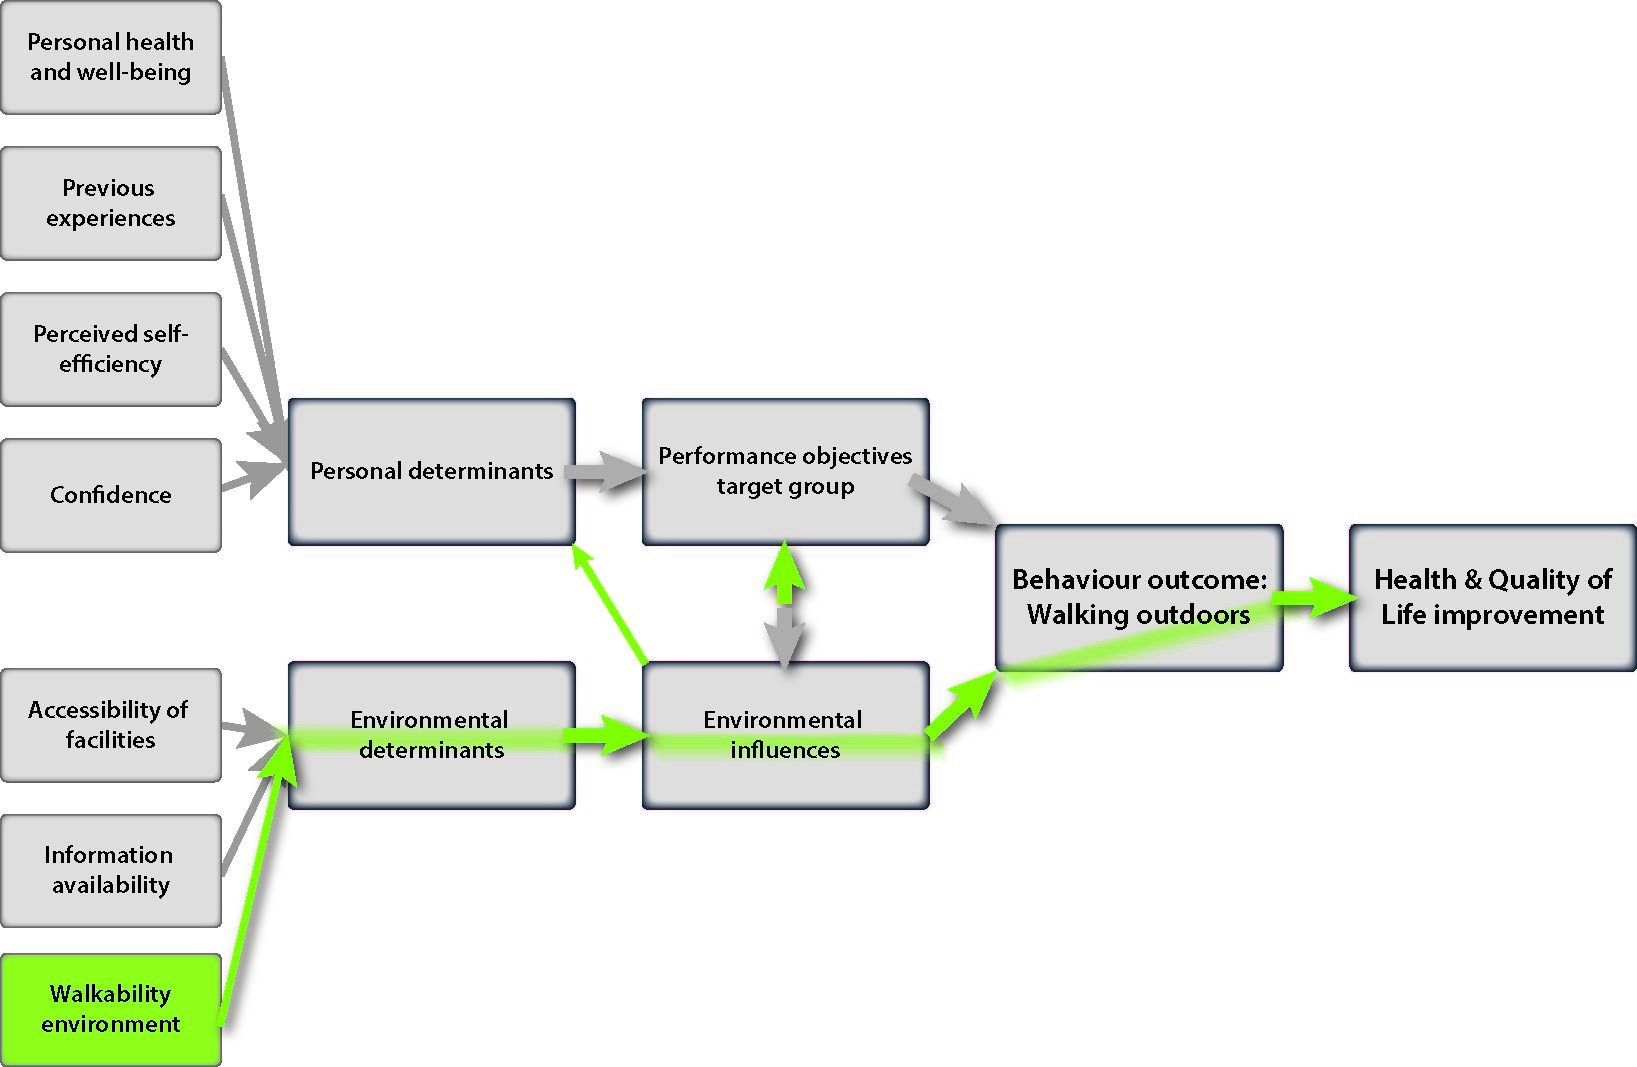
\includegraphics[width=\textwidth]{img/B_Behaviour_Scheme}
	\centering
	\caption{Walking Behaviour Scheme based on Bartholomew 2011}
	\label{behaviour}
\end{figure}


see the table \label{reffortxt} for more info.
One may readily verify that if $f$ and $g$ are continuous
functions on $D$ then the functions $f+g$, $f-g$ and
$f.g$ are continuous. If in addition $g$ is everywhere
non-zero then $f/g$ is continuous.

\end{document}
